\section{Synthèse et ouverture de l'étude}
\begin{obj}
%Objectif}
Valider le modèle de connaissance, valider la commande optimisée et envisager un prolongement à l'étude.
\end{obj}

\subsection{Validation du modèle de connaissance et de la commande optimisée}%IV.A - 
\ifprof
\else

On appelle commande optimisée la commande avec le correcteur de la boucle d'asservissement de force du type proportionnel avec limitation de la vitesse angulaire. Sur le banc d'essai avec l'actionneur linéaire, on implante ce correcteur, et on procède à quatre essais pour des consignes en échelon de force de $10,20,30$ et 40 N . Les mesures correspondantes sont tracées en traits discontinus sur la figure \ref{ccs_mp_2023_fig_22}. Ce même correcteur est mis en place dans le modèle de connaissance de la figure \ref{ccs_mp_2023_fig_11}, on obtient les réponses temporelles de simulation tracées en traits continus sur la figure \ref{ccs_mp_2023_fig_22}.

%\begin{figure}[h]
%\begin{center}
%  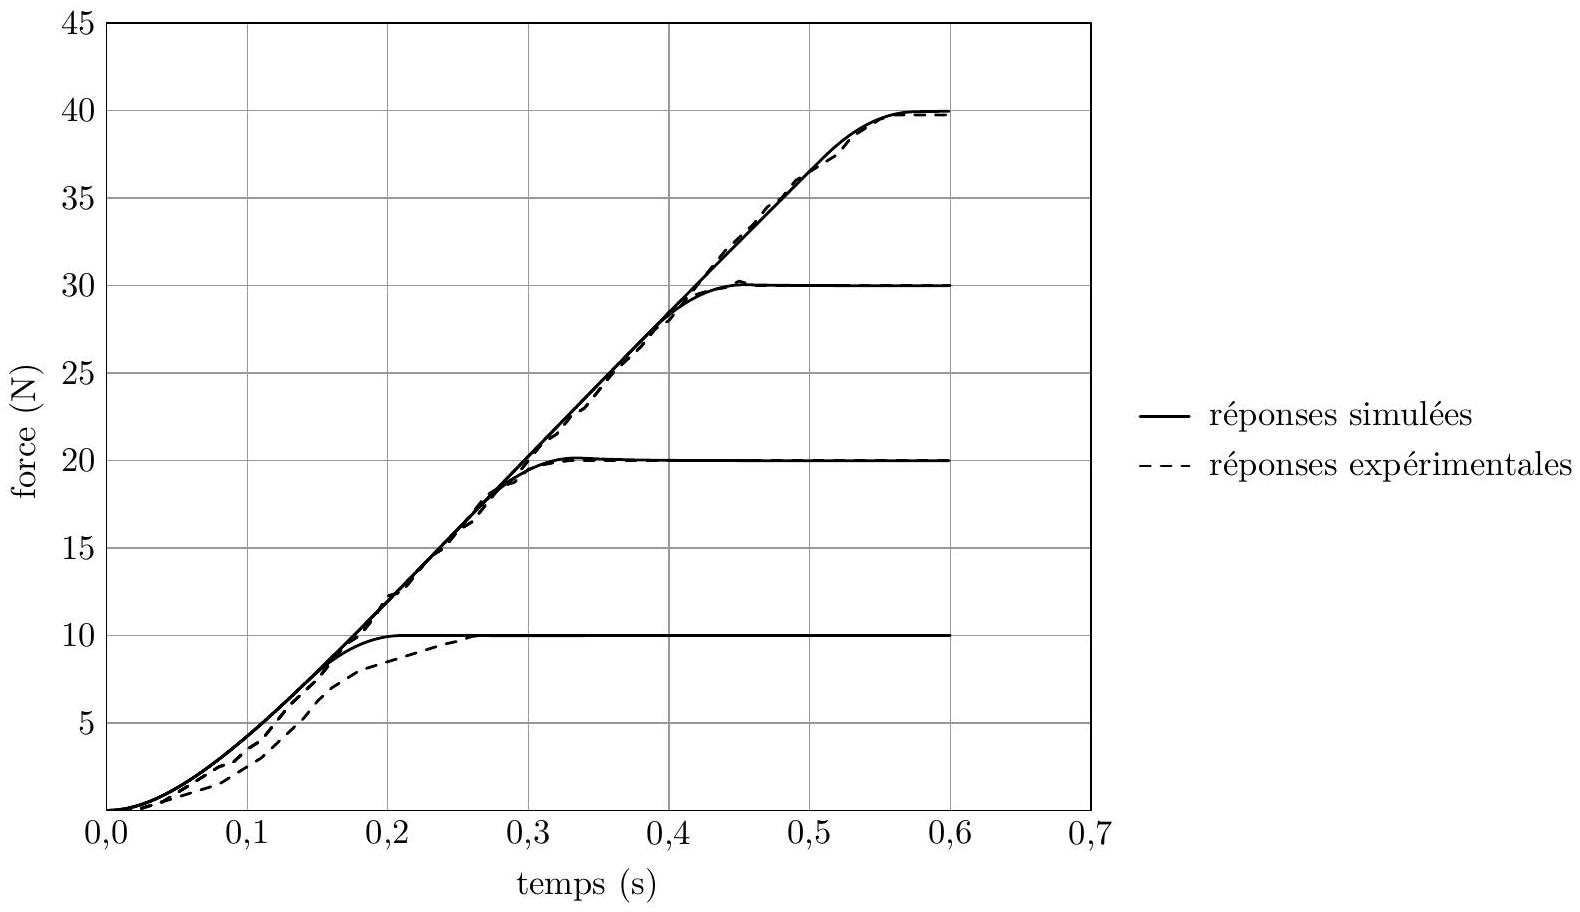
\includegraphics[width=\textwidth]{2025_09_16_5f2d7643f7e649c6833dg-15(1)}
%\captionsetup{labelformat=empty}
%\caption{Figure 22 Résultats des simulations et des expérimentations pour une entrée de consigne de force en échelon d'amplitude 10, 20,30 et 40 N}
%\end{center}
%\end{figure}

\begin{figure}[!h]
\centering
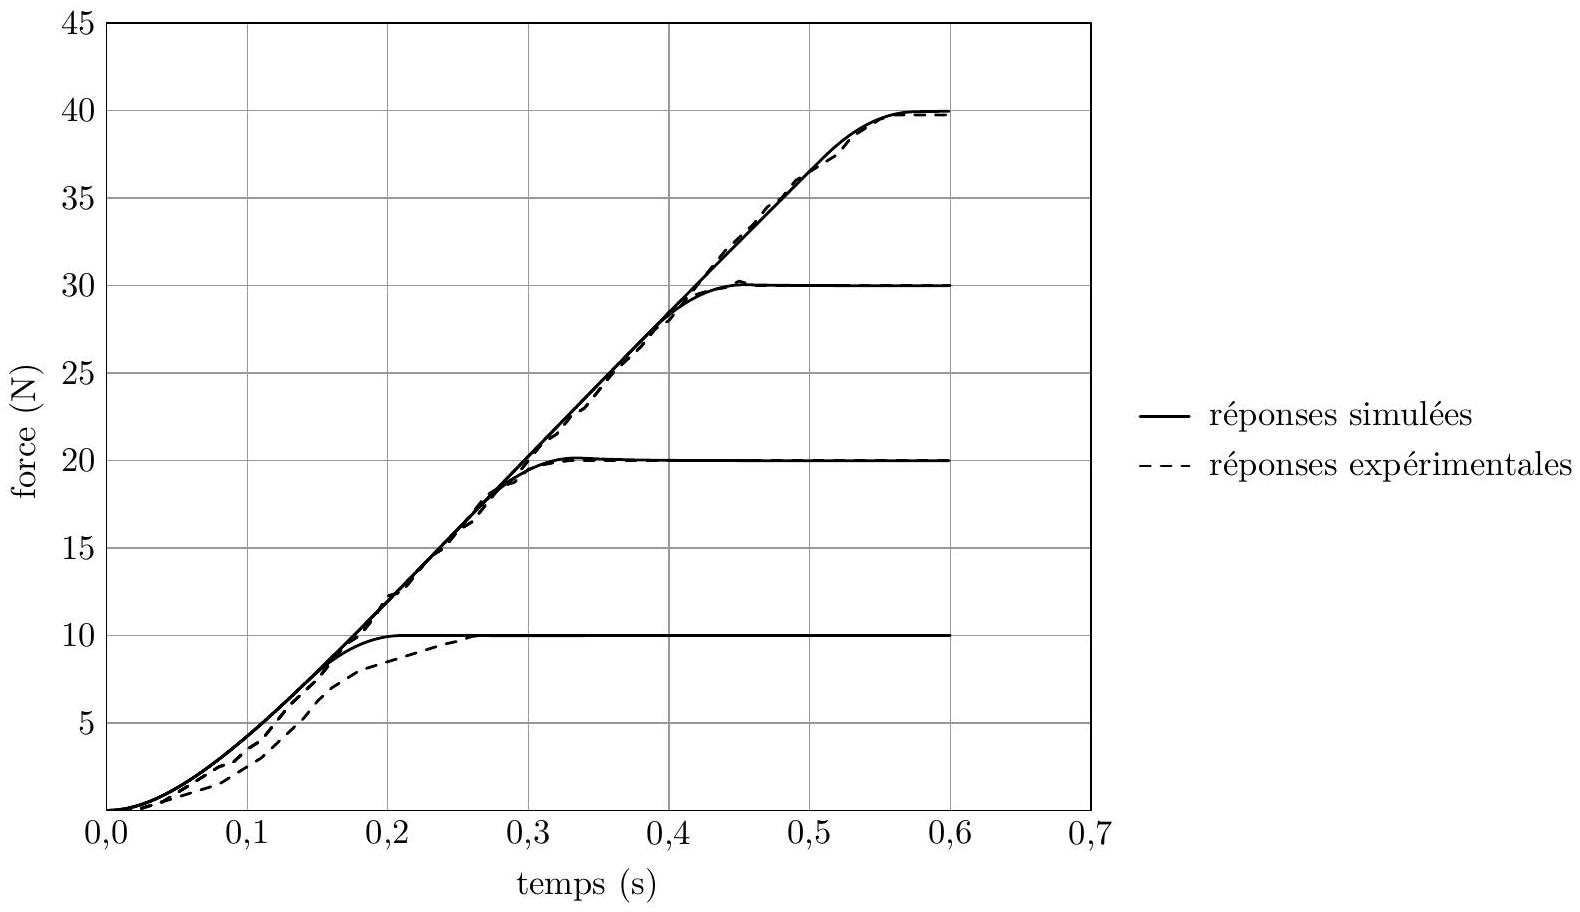
\includegraphics[width=.7\textwidth]{2025_09_16_5f2d7643f7e649c6833dg-15(1)}
\caption{\label{ccs_mp_2023_fig_22}   Résultats des simulations et des expérimentations pour une entrée de consigne de force en échelon d'amplitude 10, 20,30 et \SI{40}{N}}
\end{figure}



La démarche de l'ingénieur abordée dans le programme de sciences industrielles de l'ingénieur de la filière MP s'appuie sur les écarts entre trois performances (figure \ref{ccs_mp_2023_fig_23}).

%\begin{figure}[h]
%\begin{center}
%  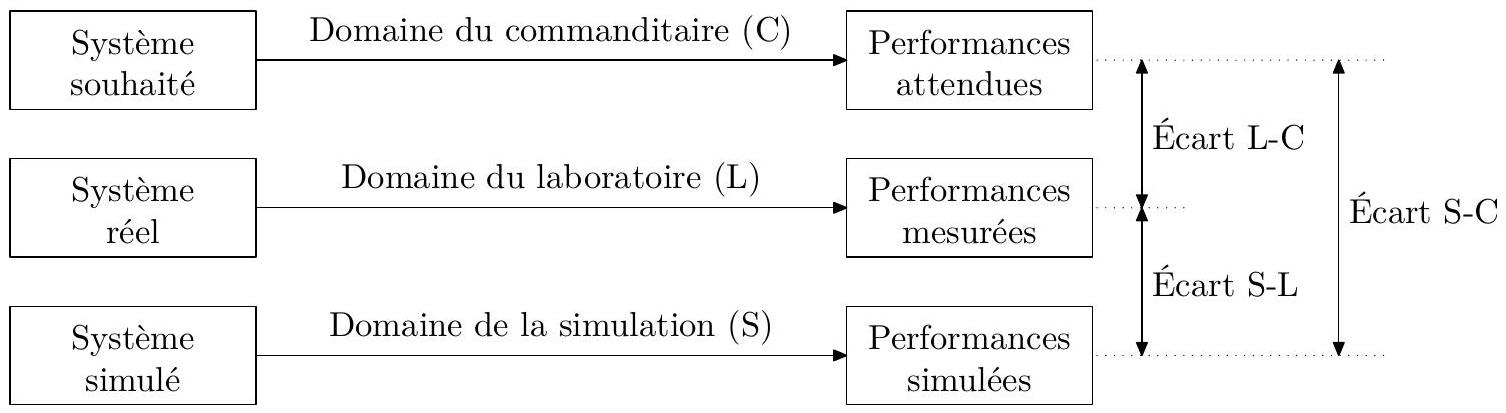
\includegraphics[width=\textwidth]{2025_09_16_5f2d7643f7e649c6833dg-15}
%\captionsetup{labelformat=empty}
%\caption{Figure 23 Synoptique de la démarche de l'ingénieur, telle que présentée dans le programme}
%\end{center}
%\end{figure}


\begin{figure}[!h]
\centering
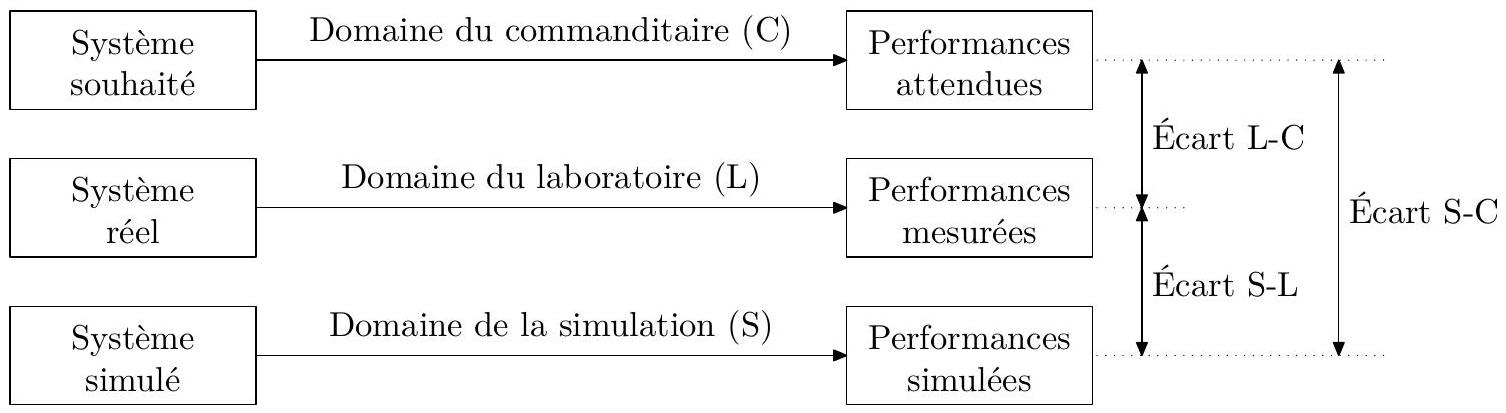
\includegraphics[width=\textwidth]{2025_09_16_5f2d7643f7e649c6833dg-15}
\caption{\label{ccs_mp_2023_fig_23}Synoptique de la démarche de l'ingénieur, telle que présentée dans le programme}
\end{figure}


En se référant à la figure \ref{ccs_mp_2023_fig_22}, l'analyse de l'écart entre les performances simulées et les performances mesurées valide le modèle de connaissance de l'asservissement de force.\\
\fi

%Q 29. 
\question{\label{ccs_mp_2023_q_29}
Choisir un des écarts L-C, S-L ou S-C permettant de valider la commande optimisée. Effectuer l'analyse de cet écart. Il est attendu une argumentation rigoureuse s'appuyant sur les données et les références du texte. Les numéros de figure, de tableau, ou d'exigence sont, par exemple, des références utilisables.}
\ifprof
\begin{corrige}
Dans ce sujet, un banc d'essais a été monté pour réaliser des expériences et une modélisation (figure \ref{ccs_mp_2023_fig_11}) basée sur ce banc d'essais a été proposée afin de prévoir les performances du système réel. Ainsi c'est l'écart S-L qui doit être analysé.\\

Sur la figure \ref{ccs_mp_2023_fig_22} on observe:
\begin{itemize}
\item[•] Consigne de 10N: il n'y a pas de dépassement ni en simulation ni en expérimentation. L'erreur statique est nulle dans les 2 cas. La vitesse de montée est plus lente lors de l'expérimentation et le temps de réponse à 5\% est plus grand (0,25s contre moins de 0,2s pour la simulation). Les frottements secs ne sont donc pas négligeables pour cette consigne, or ils n'ont pas été pris en compte dans la modélisation de la figure \ref{ccs_mp_2023_fig_11}. Les exigences de dépassement, rapidité et précision du tableau \ref{ccs_mp_2023_tab_05} sont respectées. 
\item[•] Consigne de 20N: un très léger dépassement est visible en simulation mais inférieur à 2,5\% (maximum autorisé par l'exigence de stabilité du tableau \ref{ccs_mp_2023_tab_05}), il n'y a pas de dépassement lors de l'expérience. Les observations sont similaires à celles faites pour le cas de la consigne de 10N mais le système réel met toujours un peu plus de temps à atteindre sa vitesse de montée maximale (les courbes ne se superposent bien qu'au delà de 1,15s sur la figure \ref{ccs_mp_2023_fig_22}). Le frottement sec joue encore pour cette valeur de consigne.
\item[•] Consignes de 30N et 40N: cette fois les courbes expérimentales et de simulations se superposent bien au bruit de mesure près. Le frottement sec a un effet négligeable et toutes les exigences du tableau \ref{ccs_mp_2023_tab_05} sont respectées.
\end{itemize}

Globalement la modélisation est fidèle au système réel. Afin d'améliorer le modèle on pourrait envisager de prendre en compte les effets des frottements présents dans le banc d'essais.


\end{corrige}
\else
\fi


\subsection{Étude du système perturbé}%IV.B - 

\ifprof
\else

Le schéma-blocs de la figure \ref{ccs_mp_2023_fig_24} introduit une perturbation $Y_{\text {pert }}(p)$, représentant une perturbation dans le domaine temporel $y_{\text {pert }}(t)$.

%\begin{figure}[h]
%\begin{center}
%  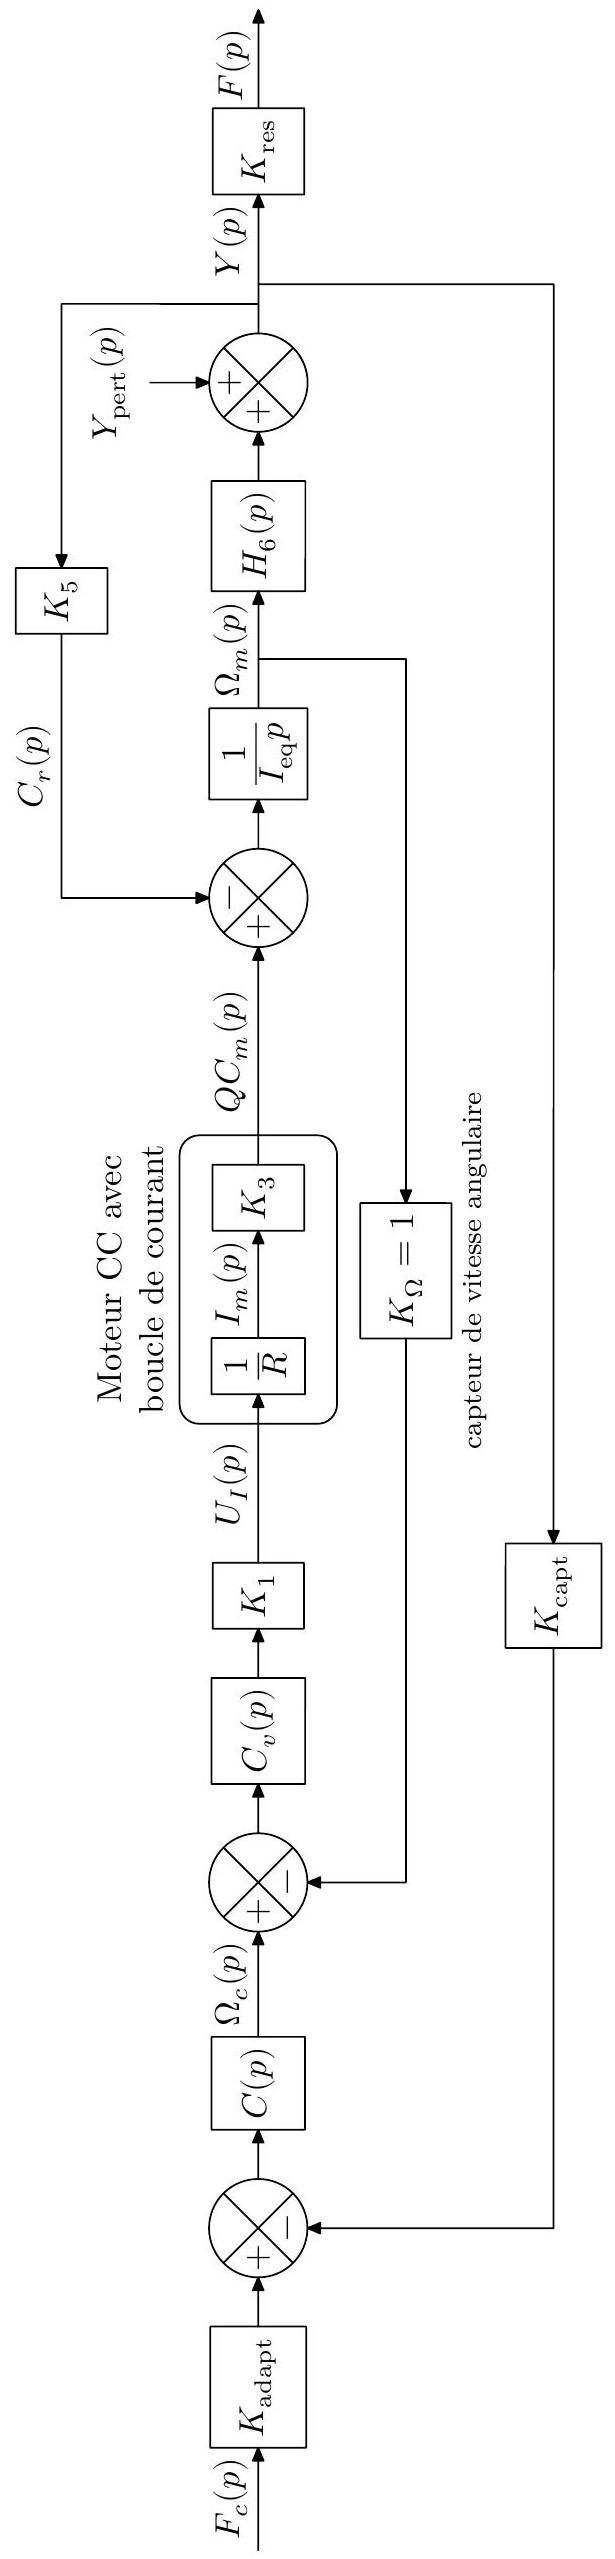
\includegraphics[width=\textwidth]{2025_09_16_5f2d7643f7e649c6833dg-16}
%\captionsetup{labelformat=empty}
%\caption{Figure 24 Schéma-blocs de l'asservissement de force développée par un actionneur linéaire avec perturbation}
%\end{center}
%\end{figure}


\begin{figure}[!h]
\centering
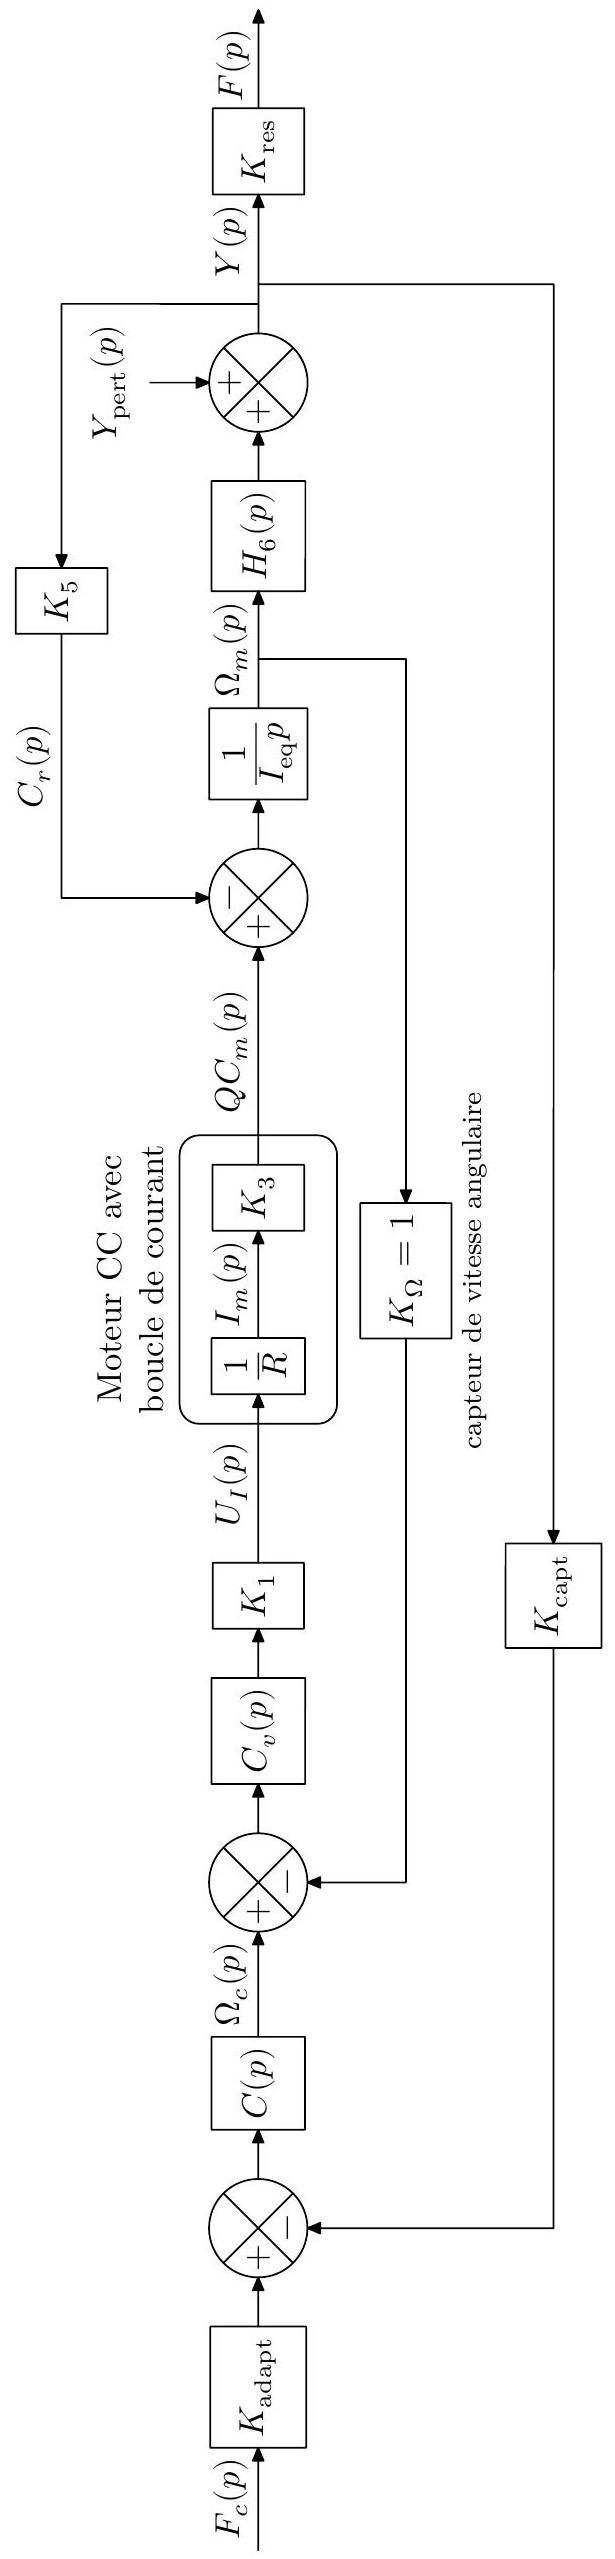
\includegraphics[width=.35\textwidth]{2025_09_16_5f2d7643f7e649c6833dg-16}
\caption{\label{ccs_mp_2023_fig_24}  Schéma-blocs de l'asservissement de force développée par un actionneur linéaire avec perturbation}
\end{figure}
\fi


%Q 30. 
\question{\label{ccs_mp_2023_q_30}
Quelle est l'unité de $y_{\text {pert}}(t)$ ? Que peut représenter cette perturbation dans le contexte de l'exosquelette lombaire? En se référant à la problématique du sujet, quel est l'intérêt d'introduire cette perturbation dans le modèle ?}
\ifprof
\begin{corrige}
$y_{\text{pert}}(t)$ est homogène à une longueur en mètres. Dans le cadre de l'exosquelette lombaire, qui s'assimile à 2 ceintures liées par des actionneurs verticaux, on peut très bien imaginer des glissements entre la ceinture et l'utilisateur ce qui peut générer des perturbations de déplacement. Il est donc nécessaire de corriger les éventuels défauts de positionnement des ceintures afin de maintenir une pression lombaire au niveau prévu par le commanditaire.
\end{corrige}
\else
\fi

\ifprof
\else

On effectue une simulation avec une perturbation normalisée représentée sur la figure \ref{ccs_mp_2023_fig_25}.

%\begin{figure}[h]
%\begin{center}
%  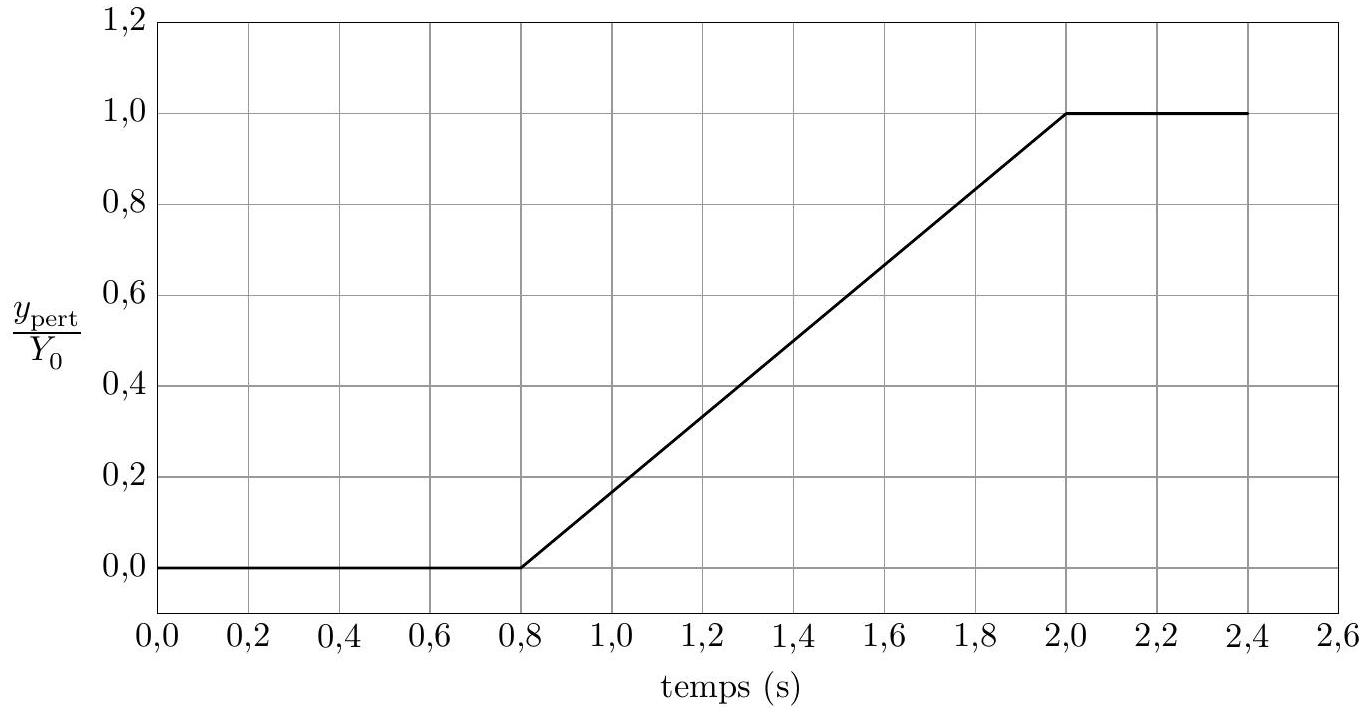
\includegraphics[width=\textwidth]{2025_09_16_5f2d7643f7e649c6833dg-17}
%\captionsetup{labelformat=empty}
%\caption{Figure 25 Évolution temporelle de la perturbation \$y\_\{\textbackslash text \{pert }\}(t)\$\}\end{center}
%\end{figure}

\begin{figure}[!h]
\centering
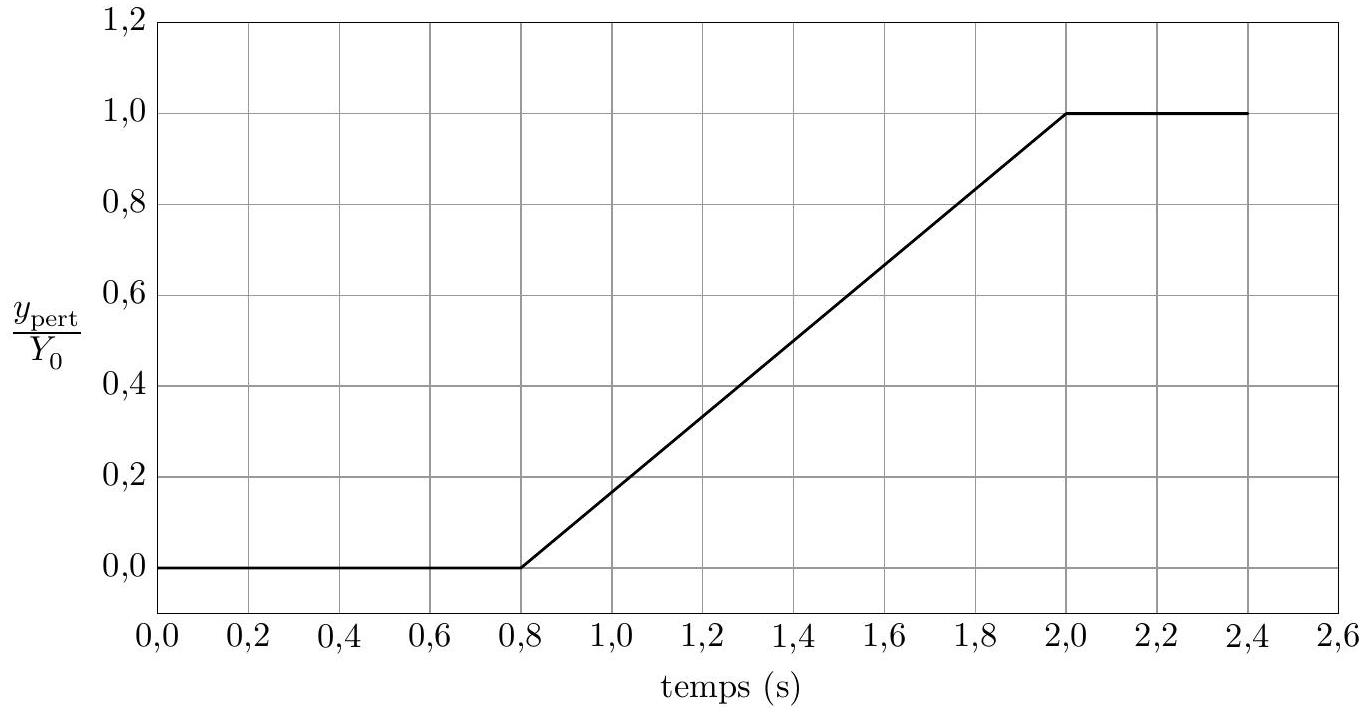
\includegraphics[width=.7\textwidth]{2025_09_16_5f2d7643f7e649c6833dg-17}
\caption{\label{ccs_mp_2023_fig_25}  Évolution temporelle de la perturbation $\indice{y}{pert}(t)$.}

\end{figure}



La figure \ref{ccs_mp_2023_fig_26} montre l'évolution de la force développée par un actionneur linéaire soumis à la perturbation décrite sur la figure \ref{ccs_mp_2023_fig_25}. C'est le résultat d'une simulation obtenue à partir du modèle de connaissance avec le correcteur proportionnel et limitation sur la vitesse angulaire.
%
%\begin{figure}[h]
%\begin{center}
%  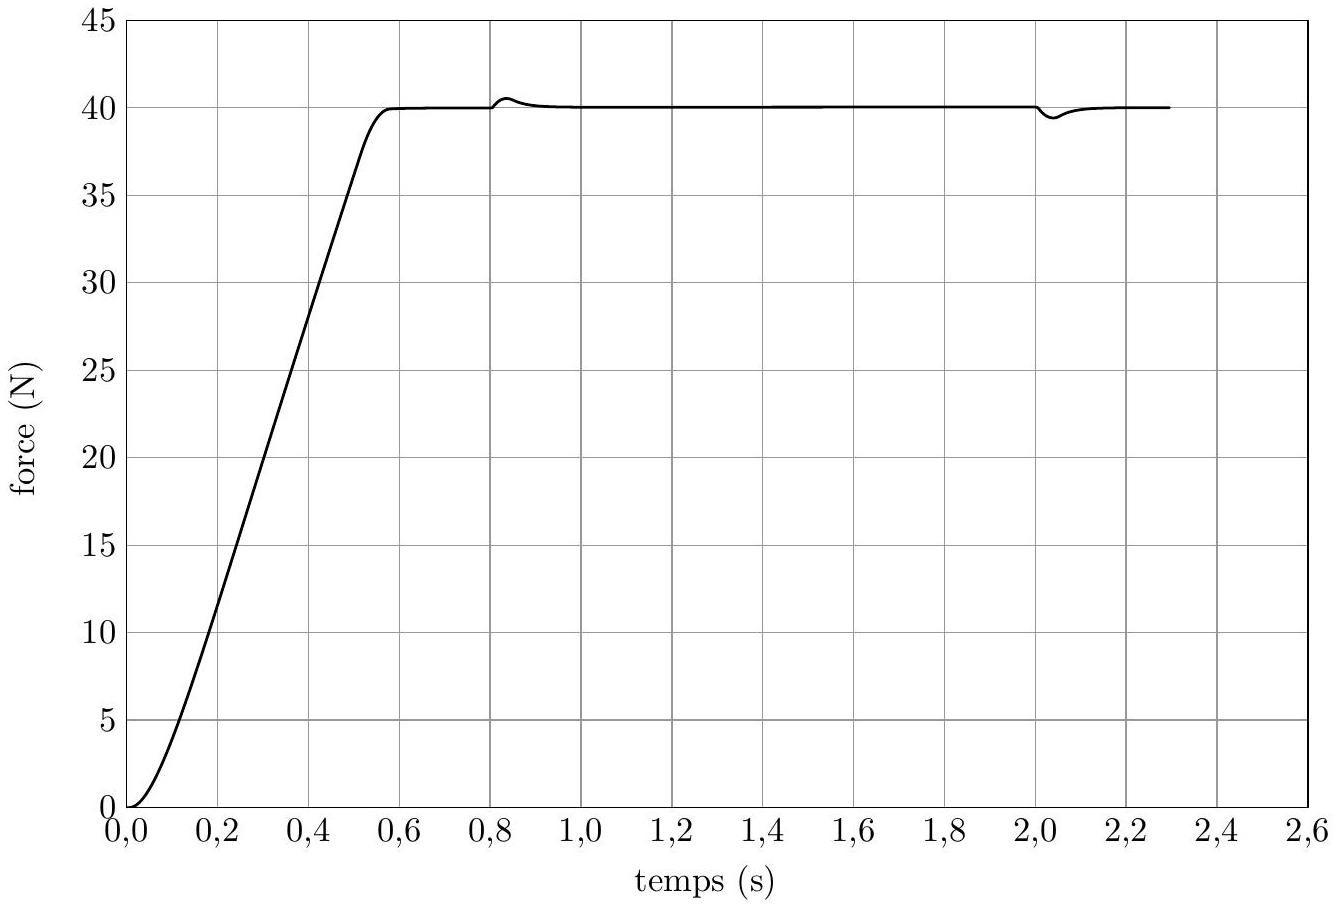
\includegraphics[width=\textwidth]{2025_09_16_5f2d7643f7e649c6833dg-17(1)}
%\captionsetup{labelformat=empty}
%\caption{Figure 26 Évolution de la force développée par l'actionneur linéaire soumis à une perturbation. Consigne en échelon de 40 N avec perturbation à \$t=0,8 \textbackslash mathrm\{\~{}s}\$\}\end{center}
%\end{figure}


\begin{figure}[!h]
\centering
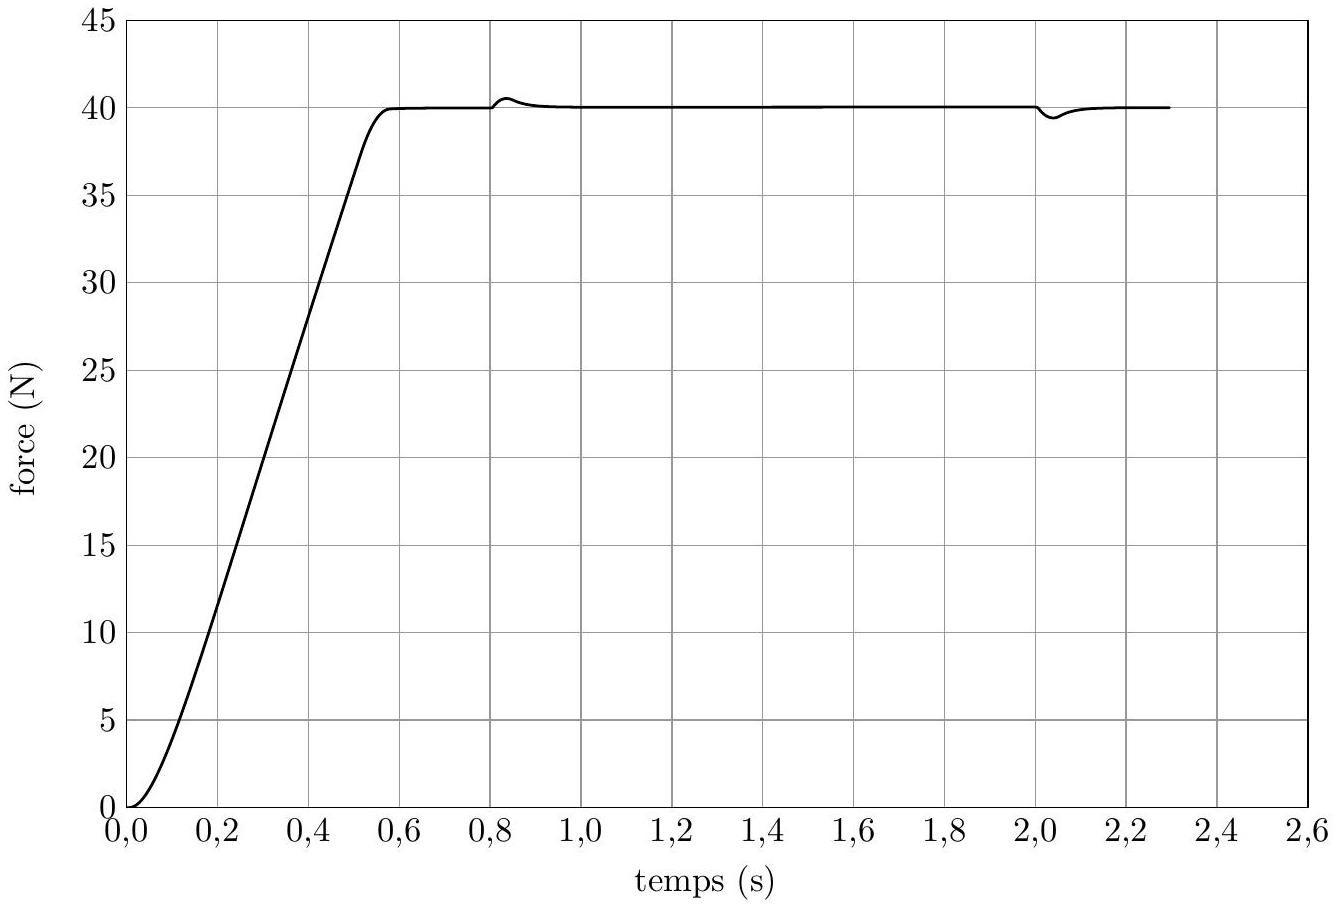
\includegraphics[width=.7\textwidth]{2025_09_16_5f2d7643f7e649c6833dg-17(1)}
\caption{\label{ccs_mp_2023_fig_26}   Évolution de la force développée par l'actionneur linéaire soumis à une perturbation. Consigne en échelon de \SI{40}{N} avec perturbation à $t=\SI{0,8}{s}$.}

\end{figure}
\fi



%Q 31. 
\question{\label{ccs_mp_2023_q_31}
Analyser la courbe de simulation de la figure \ref{ccs_mp_2023_fig_26} et conclure au regard de la problématique du sujet.}
\ifprof
\begin{corrige}
La perturbation est une fonction rampe qui démarre à partir de $t=0,8$s et devient constante à partir de $t=2$s. Si on note $u(t)$ la fonction de Heaviside on a: $y_{\text{pert}}(t) = Y_0(t-0,8)u(t-0,8) - Y_0(t-2)u(t-2)$.\\

Dans le domaine de Laplace la perturbation est en $\dfrac{1}{p^2}$ sur la partie rampe et en $\dfrac{1}{p}$ à partir de $t=0,2$s. Or dans le schéma-blocs de la figure \ref{ccs_mp_2023_fig_24} on a une double intégration en amont de la perturbation grâce aux blocs $\dfrac{1}{I_{\text{eq}}p}$ et au bloc $H_6(p)$ identifié en question \ref{ccs_mp_2023_q_15}. Le système est alors insensible à une perturbation en rampe et à une perturbation constante.\\

Cela explique les 2 "bosses" qui s'écrasent sur la figure \ref{ccs_mp_2023_fig_26}.

\end{corrige}
\else
\fi


%Q 32.
\question{\label{ccs_mp_2023_q_32}
 Le banc d'essai équipé d'un actionneur linéaire, dans la configuration étudiée dans ce sujet, permet-t-il d'analyser l'écart S-L ?}
\ifprof
\begin{corrige}
On a déjà étudié l'écart S-L en question \ref{ccs_mp_2023_q_29} puisque le modèle se basait sur le système du laboratoire. Toutefois le système du laboratoire est à l'horizontale et on a supposé en question 30 que la perturbation venait de défauts de positionnement de l'exosquelette sur l'utilisateur (donc avec les actionneurs à la verticale).\\

Enfin la proposition de perturbation de la figure \ref{ccs_mp_2023_fig_25} n'est peut-être pas réaliste. Il n'est pas possible d'évaluer un écart S-L quant à un défaut de positionnement.

\end{corrige}
\else
\fi

